% Options for packages loaded elsewhere
\PassOptionsToPackage{unicode}{hyperref}
\PassOptionsToPackage{hyphens}{url}
%
\documentclass[
]{article}
\usepackage{amsmath,amssymb}
\usepackage{lmodern}
\usepackage{ifxetex,ifluatex}
\ifnum 0\ifxetex 1\fi\ifluatex 1\fi=0 % if pdftex
  \usepackage[T1]{fontenc}
  \usepackage[utf8]{inputenc}
  \usepackage{textcomp} % provide euro and other symbols
\else % if luatex or xetex
  \usepackage{unicode-math}
  \defaultfontfeatures{Scale=MatchLowercase}
  \defaultfontfeatures[\rmfamily]{Ligatures=TeX,Scale=1}
\fi
% Use upquote if available, for straight quotes in verbatim environments
\IfFileExists{upquote.sty}{\usepackage{upquote}}{}
\IfFileExists{microtype.sty}{% use microtype if available
  \usepackage[]{microtype}
  \UseMicrotypeSet[protrusion]{basicmath} % disable protrusion for tt fonts
}{}
\makeatletter
\@ifundefined{KOMAClassName}{% if non-KOMA class
  \IfFileExists{parskip.sty}{%
    \usepackage{parskip}
  }{% else
    \setlength{\parindent}{0pt}
    \setlength{\parskip}{6pt plus 2pt minus 1pt}}
}{% if KOMA class
  \KOMAoptions{parskip=half}}
\makeatother
\usepackage{xcolor}
\IfFileExists{xurl.sty}{\usepackage{xurl}}{} % add URL line breaks if available
\IfFileExists{bookmark.sty}{\usepackage{bookmark}}{\usepackage{hyperref}}
\hypersetup{
  pdftitle={Excess Statistics},
  hidelinks,
  pdfcreator={LaTeX via pandoc}}
\urlstyle{same} % disable monospaced font for URLs
\usepackage[margin=1in]{geometry}
\usepackage{graphicx}
\makeatletter
\def\maxwidth{\ifdim\Gin@nat@width>\linewidth\linewidth\else\Gin@nat@width\fi}
\def\maxheight{\ifdim\Gin@nat@height>\textheight\textheight\else\Gin@nat@height\fi}
\makeatother
% Scale images if necessary, so that they will not overflow the page
% margins by default, and it is still possible to overwrite the defaults
% using explicit options in \includegraphics[width, height, ...]{}
\setkeys{Gin}{width=\maxwidth,height=\maxheight,keepaspectratio}
% Set default figure placement to htbp
\makeatletter
\def\fps@figure{htbp}
\makeatother
\setlength{\emergencystretch}{3em} % prevent overfull lines
\providecommand{\tightlist}{%
  \setlength{\itemsep}{0pt}\setlength{\parskip}{0pt}}
\setcounter{secnumdepth}{-\maxdimen} % remove section numbering
\ifluatex
  \usepackage{selnolig}  % disable illegal ligatures
\fi

\title{Excess Statistics}
\author{}
\date{\vspace{-2.5em}}

\begin{document}
\maketitle

\hypertarget{excess-statistics-plots-similar-to-bch}{%
\section{Excess statistics plots similar to
BCH}\label{excess-statistics-plots-similar-to-bch}}

\hypertarget{adjustment-omit}{%
\subsection{Adjustment: Omit}\label{adjustment-omit}}

\begin{verbatim}
## `summarise()` has grouped output by 'method'. You can override using the `.groups` argument.
## `summarise()` has grouped output by 'method'. You can override using the `.groups` argument.
\end{verbatim}

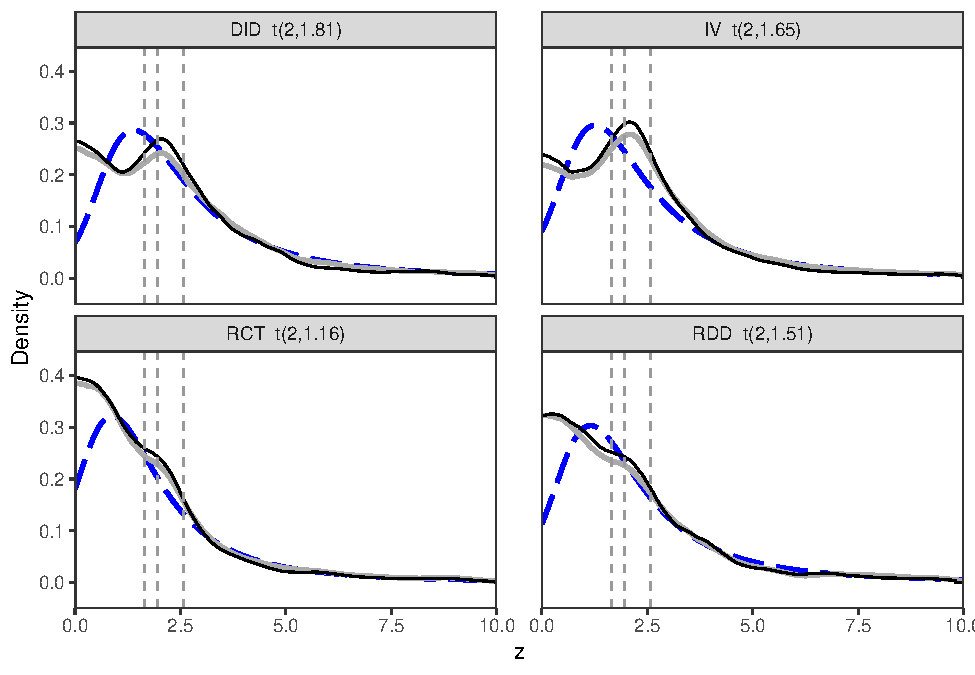
\includegraphics{C:/Users/ppuetz/Desktop/sciebo/methods_matter_replication/Submission AER/revision/comment_methods_matter/replication_repo_methods_matter_comment/Results/excess_omit-1.pdf}
Blue: Assumed t-densities from BCH Grey: z-values as reported Black:
Adjusted z-statistics

\hypertarget{biased-on-the-lhs}{%
\subsubsection{Biased on the LHS}\label{biased-on-the-lhs}}

\begin{verbatim}
## `summarise()` has grouped output by 'method'. You can override using the `.groups` argument.
## `summarise()` has grouped output by 'method'. You can override using the `.groups` argument.
\end{verbatim}

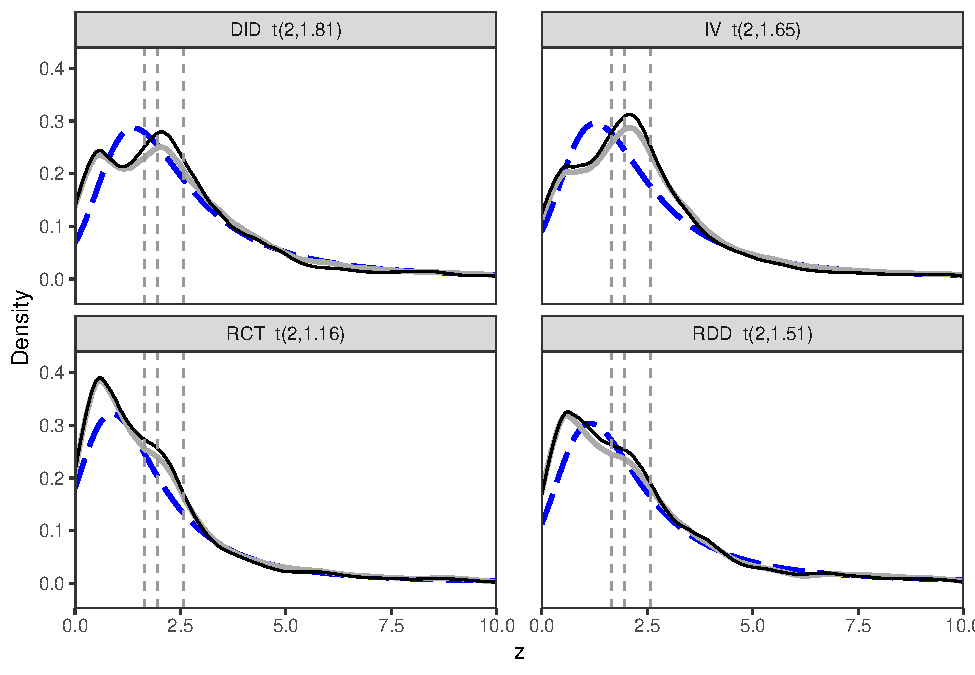
\includegraphics{C:/Users/ppuetz/Desktop/sciebo/methods_matter_replication/Submission AER/revision/comment_methods_matter/replication_repo_methods_matter_comment/Results/excess_omit_biased-1.pdf}

\hypertarget{reported-vs-t-vs-uniform}{%
\subsection{Reported vs t vs Uniform}\label{reported-vs-t-vs-uniform}}

\begin{verbatim}
## `summarise()` has grouped output by 'method'. You can override using the `.groups` argument.
## `summarise()` has grouped output by 'method'. You can override using the `.groups` argument.
\end{verbatim}

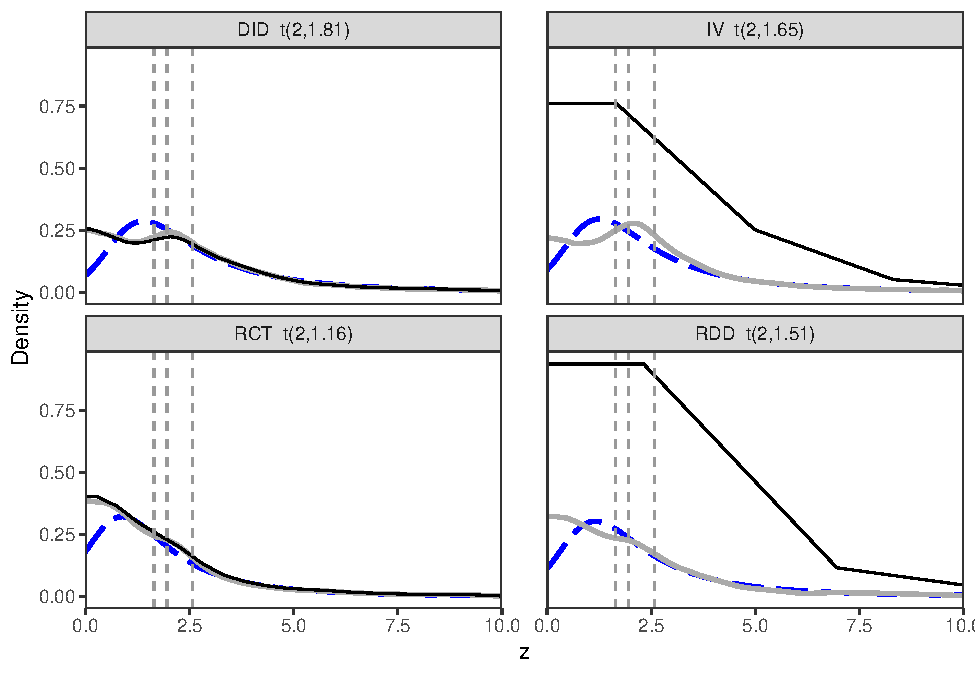
\includegraphics{C:/Users/ppuetz/Desktop/sciebo/methods_matter_replication/Submission AER/revision/comment_methods_matter/replication_repo_methods_matter_comment/Results/excess_uniform-1.pdf}
Blue: Assumed t-densities from BCH Grey: z-values as reported Black:
Adjusted z-statistics

\hypertarget{compare-with-rct}{%
\section{Compare with RCT}\label{compare-with-rct}}

\hypertarget{omit}{%
\subsection{Omit}\label{omit}}

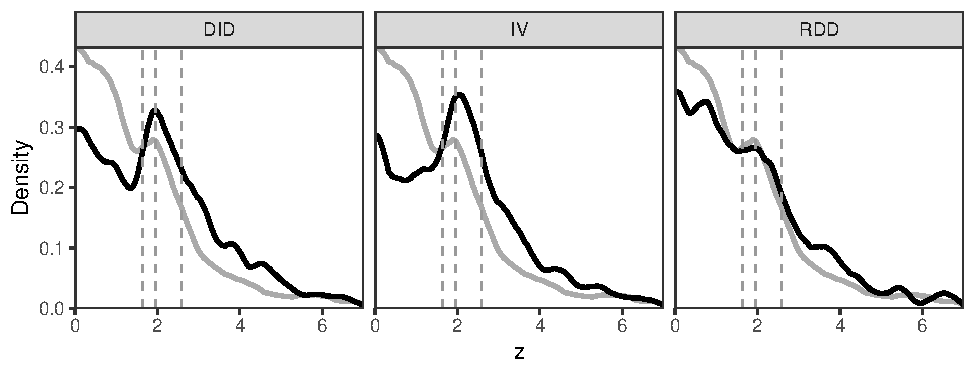
\includegraphics{C:/Users/ppuetz/Desktop/sciebo/methods_matter_replication/Submission AER/revision/comment_methods_matter/replication_repo_methods_matter_comment/Results/comp_with_rct_omit-1.pdf}

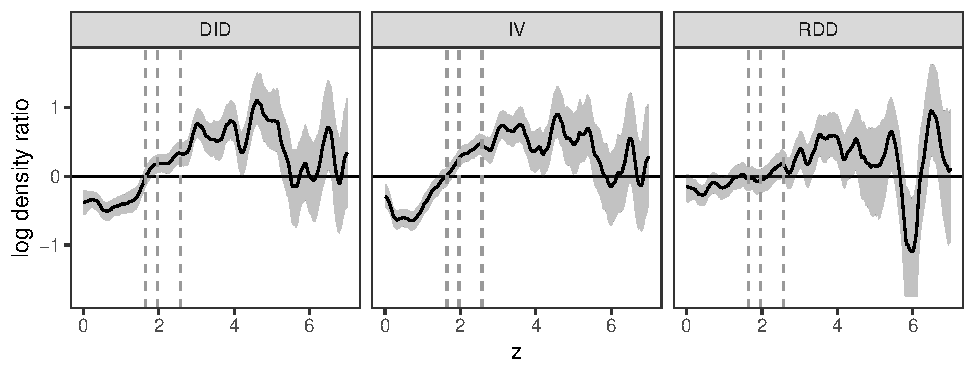
\includegraphics{C:/Users/ppuetz/Desktop/sciebo/methods_matter_replication/Submission AER/revision/comment_methods_matter/replication_repo_methods_matter_comment/Results/ratio_with_rct_omit-1.pdf}

\hypertarget{uniform-derounding}{%
\subsection{Uniform derounding}\label{uniform-derounding}}

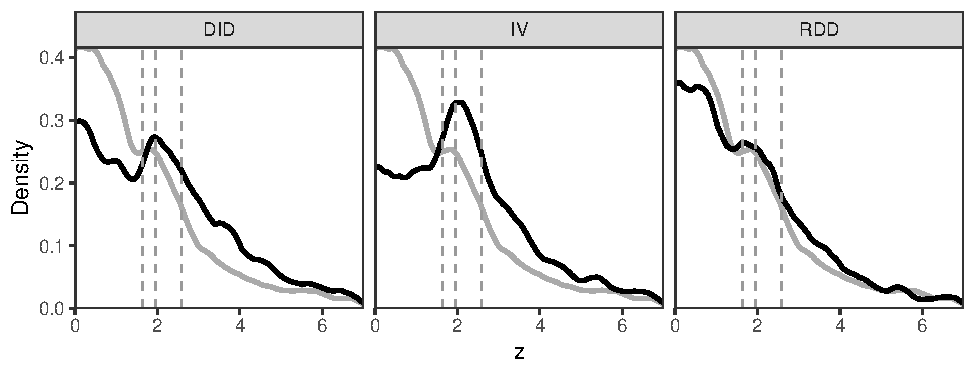
\includegraphics{C:/Users/ppuetz/Desktop/sciebo/methods_matter_replication/Submission AER/revision/comment_methods_matter/replication_repo_methods_matter_comment/Results/comp_with_rct_uniform-1.pdf}

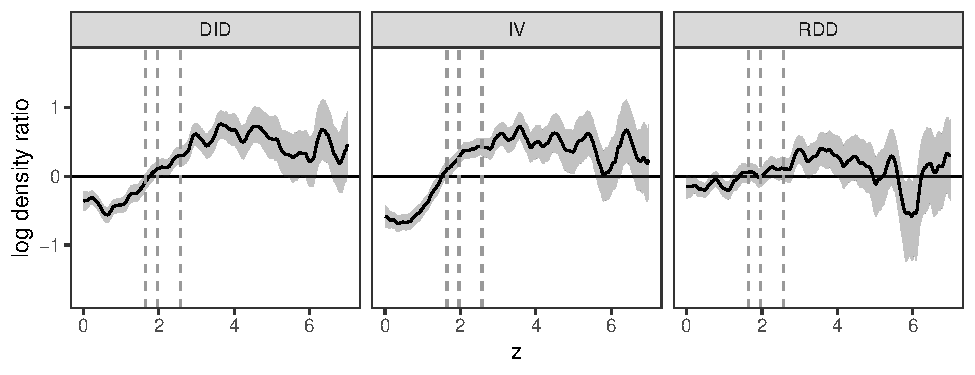
\includegraphics{C:/Users/ppuetz/Desktop/sciebo/methods_matter_replication/Submission AER/revision/comment_methods_matter/replication_repo_methods_matter_comment/Results/ratio_with_rct_uniform-1.pdf}

\hypertarget{double-hump-a-simulation}{%
\section{Double-Hump: A simulation}\label{double-hump-a-simulation}}

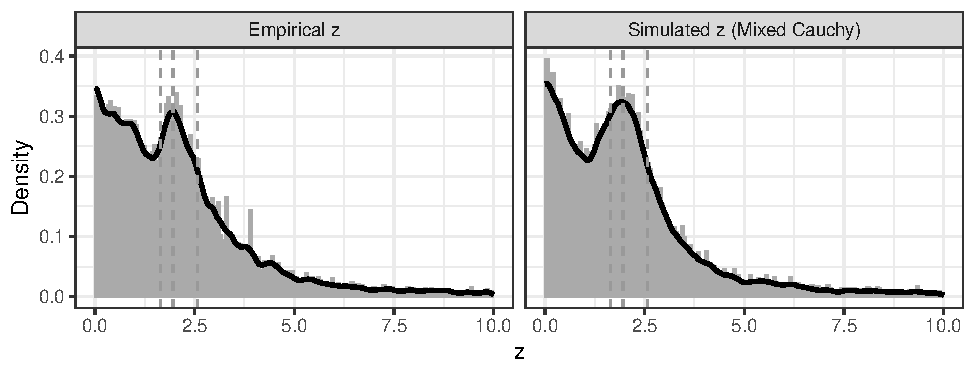
\includegraphics{C:/Users/ppuetz/Desktop/sciebo/methods_matter_replication/Submission AER/revision/comment_methods_matter/replication_repo_methods_matter_comment/Results/cauchy_sim-1.pdf}

\hypertarget{empirical-vs-t-distributions-assuming-symmetric-negative-and-positive-z}{%
\subsection{Empirical vs t-distributions assuming symmetric negative and
positive
z}\label{empirical-vs-t-distributions-assuming-symmetric-negative-and-positive-z}}

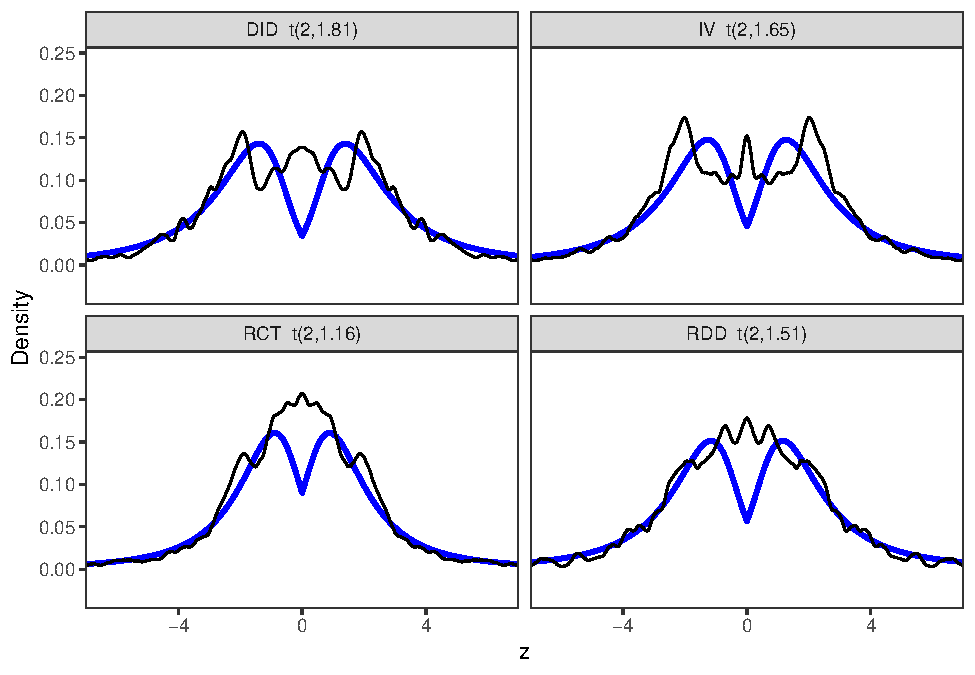
\includegraphics{C:/Users/ppuetz/Desktop/sciebo/methods_matter_replication/Submission AER/revision/comment_methods_matter/replication_repo_methods_matter_comment/Results/symmetric_t_vs_emp-1.pdf}

\hypertarget{what-probability-mass-is-below-bchs-t-curves}{%
\subsubsection{What probability mass is below BCH's
t-curves?}\label{what-probability-mass-is-below-bchs-t-curves}}

\begin{verbatim}
## [1] 0.9648521
\end{verbatim}

\begin{verbatim}
## [1] 0.9505285
\end{verbatim}

\begin{verbatim}
## [1] 0.9344783
\end{verbatim}

\begin{verbatim}
## [1] 0.8769756
\end{verbatim}

Between 87.7\% (RCT) and 96.5\% (DID)

\hypertarget{compare-with-rct_pre_registered}{%
\section{Compare with
rct\_pre\_registered}\label{compare-with-rct_pre_registered}}

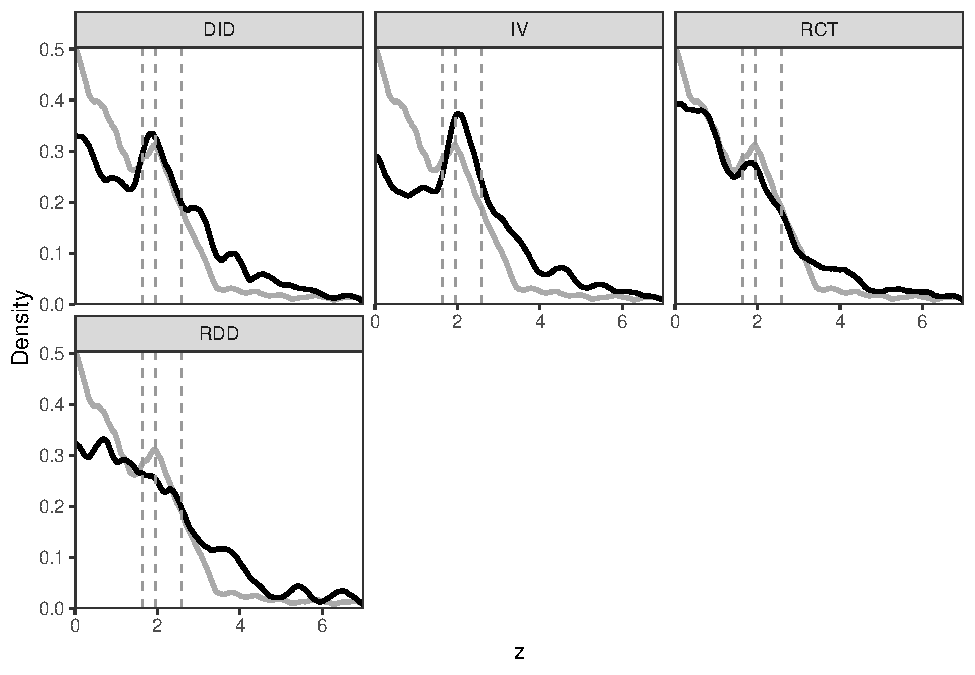
\includegraphics{C:/Users/ppuetz/Desktop/sciebo/methods_matter_replication/Submission AER/revision/comment_methods_matter/replication_repo_methods_matter_comment/Results/rct_vs_rct_registered-1.pdf}

\hypertarget{compare-density-by-year}{%
\section{Compare density by year}\label{compare-density-by-year}}

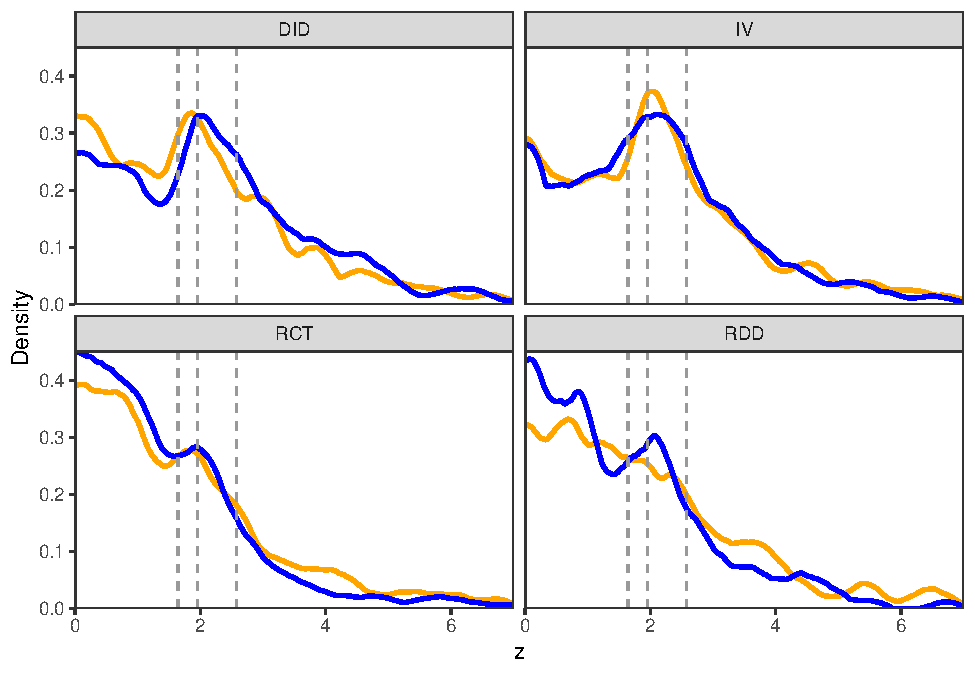
\includegraphics{C:/Users/ppuetz/Desktop/sciebo/methods_matter_replication/Submission AER/revision/comment_methods_matter/replication_repo_methods_matter_comment/Results/density_by_year-1.pdf}

\end{document}
